%%******************************************************************************
%%
%% pesqbib.tex
%%
%%******************************************************************************
%%
%% Title......: Introduction
%%
%% Author.....: GSCAR-DFKI
%%
%% Started....: Nov 2013
%%
%% Emails.....: renan028@gmail.com
%%
%% Address....: Universidade Federal do Rio de Janeiro
%%              Caixa Postal 68.504, CEP: 21.945-970
%%              Rio de Janeiro, RJ - Brasil.
%%
%%******************************************************************************


%%******************************************************************************
%% SECTION - Pesquisa Bibliográfica
%%******************************************************************************
\section{Pesquisa Bibliográfica}
\label{pesqbib}
\subsection{Stoplog}
O termo \emph{Stoplog} deriva do tempo em que eram utilizados blocos de madeira para
isolar instalações de eclusas. Atualmente, \emph{Stoplogs} são estruturas da engenharia
hidráulica utilizadas para o controle do fluxo de água de um rio, canal ou
reservatório. Essas estruturas são normalmente blocos de metal (ferro) moldados
para suportarem grande pressão hidrostática. 

\emph{Stoplogs} não podem ser posicionados livremente em grande fluxo de água, por
serem suscetíveis à vibração tanto na imersão quanto na emersão. Portanto, são guiados por trilhos no local do seu posicionamento.

Nesta seção, serão apresentadas diversas instalações que fazem proveito desta tecnologia, a sua instrumentação e sensoriamento, tipos de vedação, vantagens/desvantagens desta tecnologia, propriedades físicas do sistema, e problemas durante a instalação.  

\paragraph{Santa Clara River}\mbox{}\\
Localizado na Califórnia, as principais áreas que contornam o rio Santa Clara
são: Ventura Road, Strouble Drain, Wagonwheel Shopping Center e Mobile Home
Park, áreas 285-1, 285-2 e 285-3, respectivamente, da figura~\ref{pesqbib_1}.

\begin{figure}[H]
    \centering
    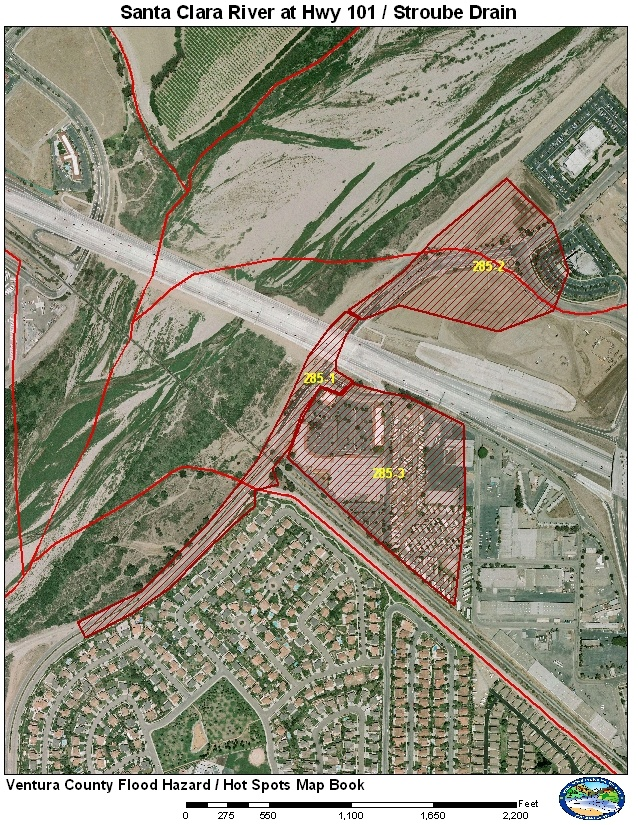
\includegraphics[width=0.5\columnwidth]{figs/pesqbib/1.jpg}
    \caption{Mapa da região do rio Santa Clara}
    \label{pesqbib_1}
\end{figure}
 
Em janeiro de 2005, o rio atingiu um fluxo de 3851 $m^3/s$, alagando as regiões
da Venture Road e comprometendo Strouble Drain. A partir de então, houve
investimento na construção de portas hidráulicas para medir o fluxo do rio. 

 \emph{Stoplogs} foram uma solução em Strouble Drain para prevenir inundações em Riverpark. Porém, pode haver problemas quando um fluxo muito grande de água não é drenado, causando inundação de áreas vizinhas. Portanto, Strouble deve ser observado durante o alto fluxo, pois pode haver reversão do fluxo da água. O processo de inserção de  \emph{Stoplogs} é realizado manualmente por guindaste e demora em torno de 3 horas.

\paragraph{River Great Ouse}\mbox{}\\
Localizado em King’s Lynn, na Inglaterra, o rio Ouse sofria problemas de inundações mesmo após 1988, quando foi instalada uma porta hidráulica de 16m. Em agosto de 2006, houve a construção de um novo sistema de defesa utilizando sete  \emph{Stoplogs} 16mx9m com 7.5 toneladas cada. Em Alexandra Dock, porto comercial de King’s Lynn, os \emph{Stoplogs} são erguidos por guindastes móveis.

\begin{figure}[H]
    \centering
    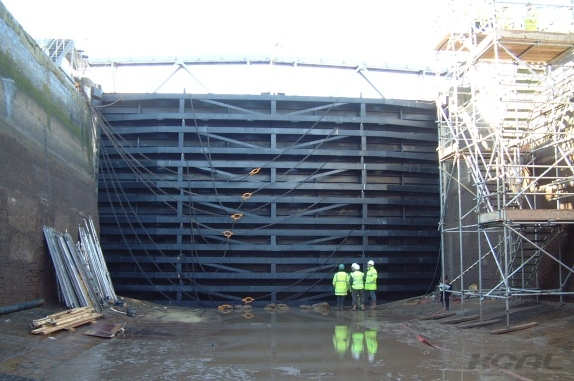
\includegraphics[width=1\columnwidth]{figs/pesqbib/2.jpg}
    \caption{Stoplog em River Great Ouse}
    \label{pesqbib_2}
\end{figure}
 
Os três últimos \emph{Stoplogs}, que formam a base, apresentam quatro válvulas
tipo flap não retornáveis para reduzir o nível do rio
Ouse, como observado na figura
\ref{pesqbib_2}.

\paragraph{Lakefield Generating Station}\mbox{}\\
Em 1928, Lakefield, Canada, foi construída a planta de geração de energia no rio
de Ontario, Otonabee River. A água passa por quatro comportas de 6 m até uma
guia de adução, parede de concreto de 533.4 m para direcionar a água até a casa
de energia. Essas comportas podem ser fechadas com \emph{Stoplogs} quadrados de 
madeira de 35.6 cm. Da guia de adução, a água é direcionada até três comportas 
de 4.3 m de comprimento também equipadas com \emph{Stoplogs} e chega na
turbina, como observado na figura \ref{pesqbib_3}.

\begin{figure}[H]
    \centering
    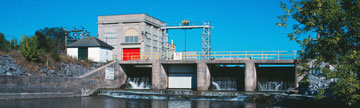
\includegraphics[width=1\columnwidth]{figs/pesqbib/3.jpg}
    \caption{Lakefield Generating Station}
    \label{pesqbib_3}
\end{figure}
 
\paragraph{Killaloe Canal}\mbox{}\\
Localizado no rio Shannon, Irlanda, o canal de Killaloe é passagem de embarcações de pequeno porte. O canal, porém, 
tornou-se redundante em 1929 com a instalação da hidrelétrica de Ardnacrusha devido ao aumento do nível do rio. Dessa forma, 
novas portas foram instaladas no local e, para assistir a instalação e futura
manutenção, dois conjuntos de \emph{Stoplogs} de ferro serão utilizados, como
observado na figura \ref{pesqbib_4}.

\begin{figure}[H]
    \centering
    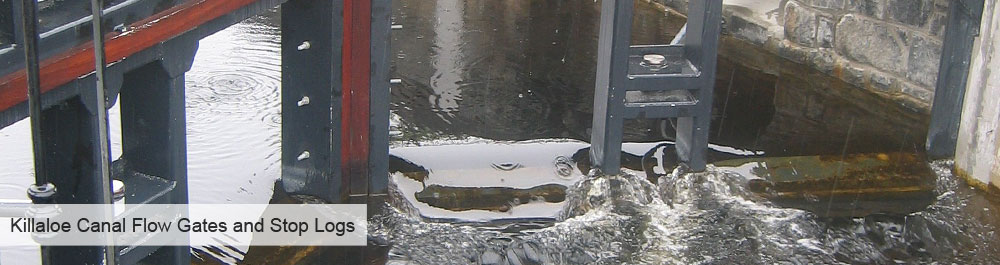
\includegraphics[width=1\columnwidth]{figs/pesqbib/4.jpg}
    \caption{Killaloe Canal}
    \label{pesqbib_4}
\end{figure}   

\paragraph{The Goolwa Barrage}\mbox{}\\
Localizado na Austrália, Goolwa compreende cinco barragens que ligam o 
lago Alexandrina e o rio Murray Mouth. O controle do nível da água é 
realizado tipicamente com \emph{Stoplogs} e pequeno número de portas r
adiais e automáticas, com ilustrado na figura \ref{pesqbib_5}. 
Períodos de baixo fluxo de água no rio, \emph{Stoplogs} e portas fecham 
completamente o fluxo e assiste em manter o nível do lago. Em casos de inundações , \emph{Stoplogs} são removidos e as portas hidráulicas são abertas.
 

\begin{figure}[H]
    \centering
    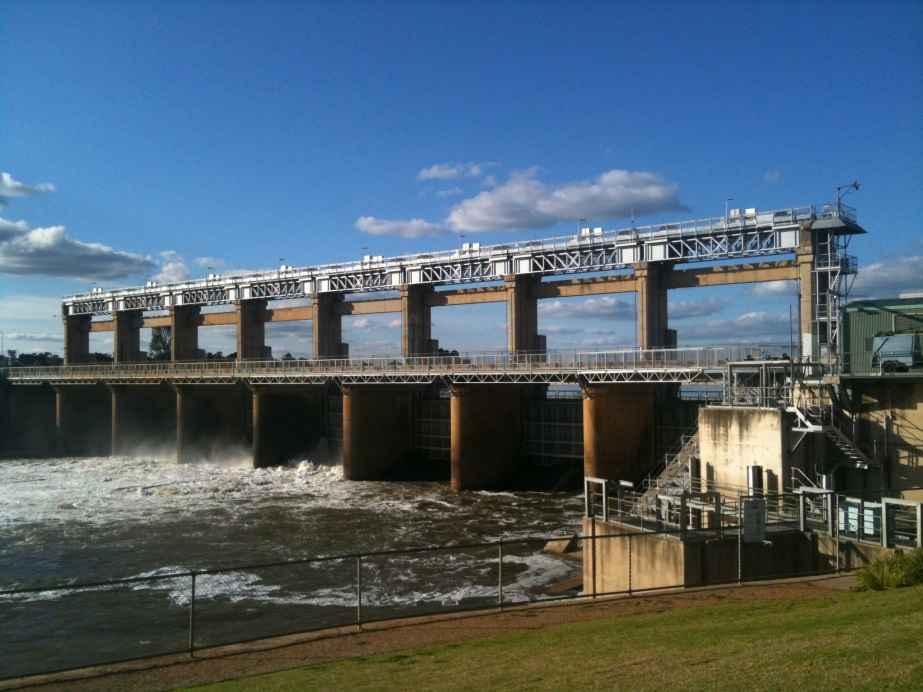
\includegraphics[width=0.8\columnwidth]{figs/pesqbib/6.jpg}
    \caption{The Goolwa Barrage}
    \label{pesqbib_5}
\end{figure}   
 
\paragraph{Conclusão das aplicações}\mbox{}\\
\emph{Stoplogs} são utilizados com ampla finalidade: controle de nível d’água do rio para prevenir inundações, regular nível para a reutilização de comportas em rios que sofreram grande variação de fluxo devido a hidrelétricas, bloquear fluxo d’água para construção de barragens e manutenção, reduzir fluxo de água para turbinas.
As vantagens na utilização desta tecnologia são:
\begin{itemize}
\item Provê excelente controle de nível de água e drenagem.
\item Ajustável ao nível da água desejado: empilhamento e válvulas flap.
\item Baixa manutenção.
\item Fabricação e projeto são normalmente de baixo custo.
\item Pode ser fixado no local ou móvel.
\end{itemize}

As desvantagens na utilização desta tecnologia são:
\begin{itemize}
  \item Pode apresentar vazamento.
  \item Difícil remoção em caso de grande pressão hidrostática.
  \item Operados manualmente.
  \item Restritivo à passagem de peixes.
  \item Não há proteção contra inundações acima do último \emph{Stoplog}.
  \item Facilmente adulterado ou vandalizado.
  \item Pode requerer infraestrutura com proteção adicional devido à manipulação
  de objetos de grande porte.
\end{itemize}

\paragraph{Propriedades físicas, instrumentação e sensoriamento de
\emph{Stoplogs}}\mbox{}\\ Jack Lewin, em seu livro Hydraulic Gates and Valves: In Free Surface Flow and Submerged Outlets, estuda as propriedades de um \emph{Stoplog} e \emph{Lifting Beam} semelhantes aos utilizados no projeto ROSA. 
Na figura~\ref{pesqbib_7}, pode ser observada a vedação inferior ‘a’ e superior
‘b’ do \emph{Stoplog}, e uma válvula ‘d’ conectada ao olhal de tal forma que ao encaixar o \emph{Lifting Beam} e início de movimento, a válvula é aberta para igualar a pressão hidrostática da parte superior com a inferior do \emph{Stoplog}. O sensor de contato mecânico (haste) ‘e’, no \emph{Stoplog}, é posicionado na parte inferior ou superior. O deslocamento da haste permite o desencaixe da garra.

\begin{figure}[H]
    \centering
    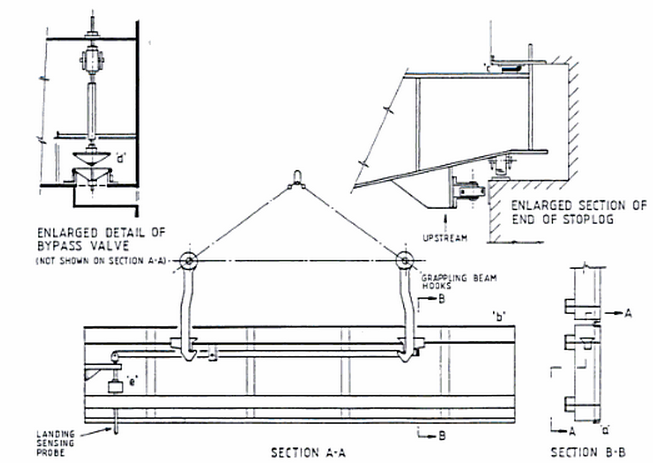
\includegraphics[width=1\columnwidth]{figs/pesqbib/7.png}
    \caption{Stoplog de Jack Lewin}
    \label{pesqbib_7}
\end{figure} 

\begin{figure}[H]
    \centering
    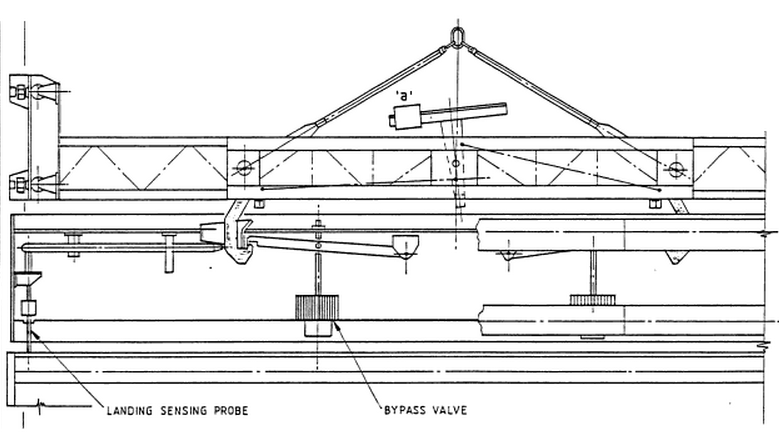
\includegraphics[width=1\columnwidth]{figs/pesqbib/8.png}
    \caption{Stoplog de Jack Lewin}
    \label{pesqbib_8}
\end{figure}  
 
Apesar de possuir design semelhante, o \emph{Stoplog} a ser utilizado no projeto ROSA não é instrumentado como o modelo estudado por Jack Lewin. O sensor de mecânico de contato, acoplado à haste que realiza o desencaixe, e a válvula reguladora de pressão hidrostática não estão disponíveis na versão simplificada do \emph{Stoplog} do projeto.

Em Design of Movable Weirs and Storm Surge Barries: Report of Working Group 26,
a Inglaterra busca a padronização de \emph{Stoplogs} por razões de fabricação, 
econômica e manutenção. Em Lagan, Irlanda do Norte, os \emph{Stoplogs} são padronizados 
e as portas hidráulicas foram construídas de tal forma a suportar a estrutura. 
Os \emph{Stoplogs} têm 13,8m de comprimento, 1,25 m de espessura e pesam 7018 kg. 
Esses e outros \emph{Stoplogs} utilizados no Reino Unido não apresentam, porém,
os sensores descritos por Jack Lewin. 

Em Ivanhoe River 2009, em Ontario, Canada, \emph{Stoplogs} sem sensoriamento foram 
instalados para o controle do fluxo do rio. A fim de não alterar a estrutura do \emph{Stoplog}, 
a solução da empresa Hatch ficou responsável pelo desenvolvimento de um \emph{Lifting Beam} 
para monitoramento da operação. As garras foram instrumentadas com sensores indutivos 
para monitorar o contato, além de serem independentemente atuadas. A figura
\ref{pesqbib_9} ilustra o \emph{Lifiting Beam} desenvolido pela Hatch.

\begin{figure}[H]
    \centering
    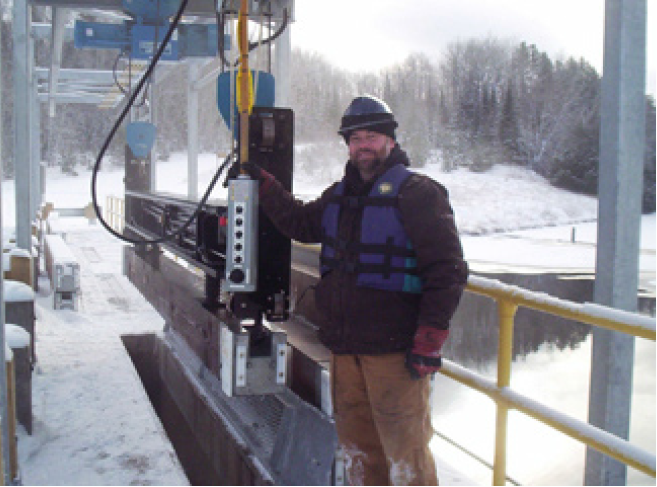
\includegraphics[width=0.5\columnwidth]{figs/pesqbib/9.png}
    \caption{Lifting Beam da Hatch}
    \label{pesqbib_9}
\end{figure}  
 
 
Outra solução semelhante, que realiza a instrumentação no \emph{Lifting Beam}, foi utilizada pela Atlaspolar.
Da mesma forma, sensores indutivos e de força são acoplados ao \emph{Lifting
Beam}. O processo requer diversos \emph{Stoplogs}, o que inviabiliza sua instrumentação 
pelo custo e, principalmente, por corrosão e danos por impacto, vibração. A
figura \ref{pesqbib_10} ilustra o \emph{Lifiting Beam} utilizado pela
Atlaspolar.

\begin{figure}[H]
    \centering
    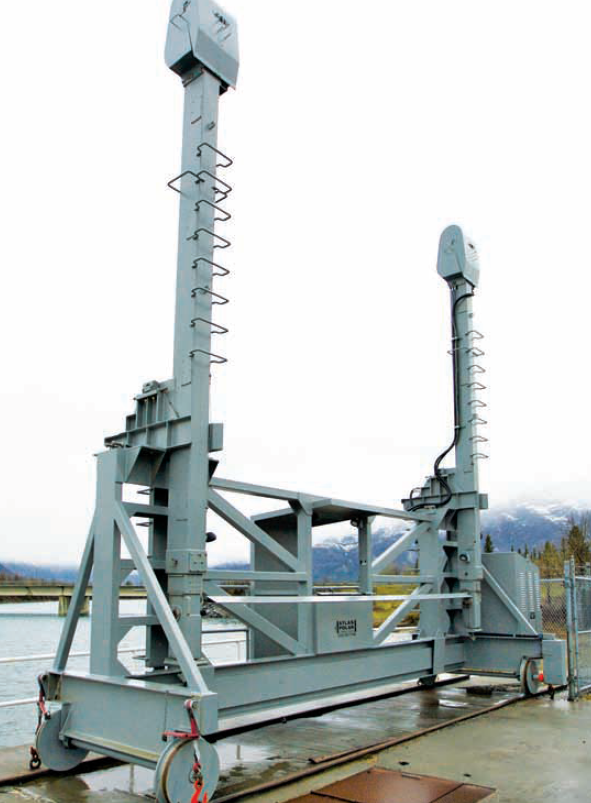
\includegraphics[width=0.5\columnwidth]{figs/pesqbib/10.png}
    \caption{Lifting Beam da Atlaspolar}
    \label{pesqbib_10}
\end{figure}   

A manutenção de \emph{Stoplogs} é realizada fazendo-se a inspeção da região de vedação, área de contato entre \emph{Stoplogs}. Esta área perde a pintura e é de fácil localização, sendo realizada, normalmente, anualmente.
